% ============================================================
\chapter{Mod\`eles ARIMA et Diff\'erenciation}
\label{ch:arima}
% ============================================================

\section{Exemple motivant}
Le PIB trimestriel fran\c{c}ais pr\'esente une tendance croissante : il n'est pas stationnaire. Apr\`es une diff\'erenciation ($\nabla X_t = X_t - X_{t-1}$), le taux de croissance est approximativement stationnaire et mod\'elisable par un ARMA.

\section{Processus int\'egr\'es}\index{processus integre@processus int\'egr\'e}

\begin{definition}[Processus int\'egr\'e d'ordre $d$]
$(X_t)$ est \textbf{int\'egr\'e d'ordre $d$}, not\'e $X_t\sim I(d)$, si $\nabla^d X_t = (1-B)^d X_t$ est stationnaire mais $\nabla^{d-1}X_t$ ne l'est pas.
\end{definition}

\begin{exemple}
La marche al\'eatoire $X_t=X_{t-1}+\eps_t$ est $I(1)$ car $\nabla X_t = \eps_t$ est stationnaire.
\end{exemple}

\section{Mod\`ele ARIMA$(p,d,q)$}\index{ARIMA}

\begin{definition}[ARIMA$(p,d,q)$]
\[
\phi(B)(1-B)^d X_t = \theta(B)\eps_t.
\]
$X_t$ suit un ARIMA$(p,d,q)$ si $W_t = \nabla^d X_t$ suit un ARMA$(p,q)$.
\end{definition}

\begin{attention}
On diff\'erencie pour rendre stationnaire, mais \textbf{trop diff\'erencier} ($d$ trop grand) introduit des racines MA proches du cercle unit\'e, ce qui d\'egrade les pr\'evisions. En pratique, $d\leq 2$.
\end{attention}

\section{SARIMA : saisonnalit\'e}\index{SARIMA}

\begin{definition}[SARIMA$(p,d,q)\times(P,D,Q)_s$]
Pour une s\'erie de p\'eriode $s$ :
\[
\Phi(B^s)\phi(B)(1-B)^d(1-B^s)^D X_t = \Theta(B^s)\theta(B)\eps_t,
\]
o\`u $\Phi$, $\Theta$ sont les polyn\^omes saisonniers d'ordres $P$, $Q$.
\end{definition}

\begin{exemple}[Airline model]
Le mod\`ele de Box--Jenkins pour AirPassengers est un SARIMA$(0,1,1)\times(0,1,1)_{12}$ :
\[
(1-B)(1-B^{12})X_t = (1+\theta_1 B)(1+\Theta_1 B^{12})\eps_t.
\]
\end{exemple}

\section{Strat\'egie de diff\'erenciation}

\begin{methode}
\begin{enumerate}
\item Tracer la s\'erie et son ACF. Si l'ACF d\'ecro\^it tr\`es lentement, diff\'erencier.
\item Appliquer le test ADF (ou KPSS). Si $H_0$ (racine unitaire) n'est pas rejet\'ee, diff\'erencier.
\item Apr\`es diff\'erenciation, v\'erifier que la s\'erie r\'esultante est stationnaire.
\item Pour la saisonnalit\'e, diff\'erencier \`a l'ordre $s$ si l'ACF montre des pics p\'eriodiques.
\end{enumerate}
\end{methode}

\section{Exemple num\'erique : AirPassengers}

\begin{center}
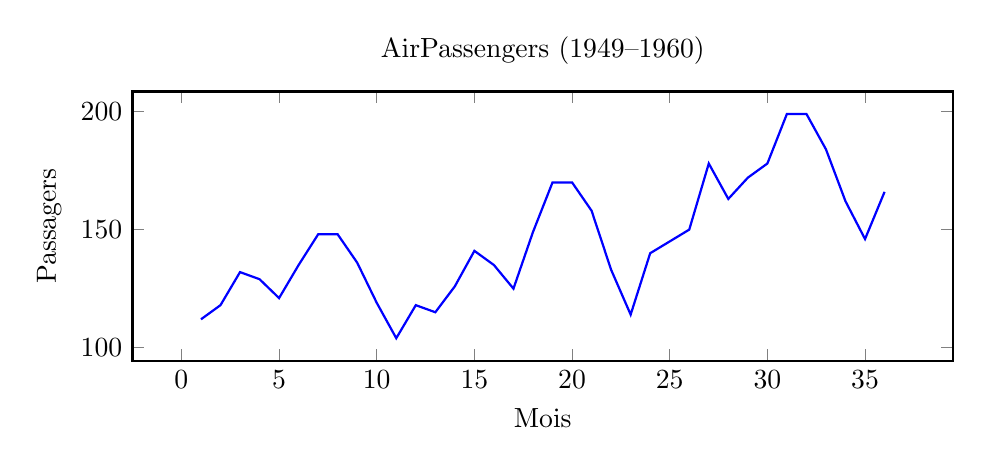
\begin{tikzpicture}
\begin{axis}[
  width=12cm, height=5cm, xlabel={Mois}, ylabel={Passagers},
  title={AirPassengers (1949--1960)}, no markers, thick
]
\addplot[blue] coordinates {
(1,112)(2,118)(3,132)(4,129)(5,121)(6,135)(7,148)(8,148)(9,136)
(10,119)(11,104)(12,118)(13,115)(14,126)(15,141)(16,135)(17,125)
(18,149)(19,170)(20,170)(21,158)(22,133)(23,114)(24,140)
(25,145)(26,150)(27,178)(28,163)(29,172)(30,178)(31,199)(32,199)
(33,184)(34,162)(35,146)(36,166)
};
\end{axis}
\end{tikzpicture}
\end{center}

\section{Impl\'ementation}

\begin{codeblock}[title=\textbf{Python}]
\begin{minted}{python}
import numpy as np
import pandas as pd
import matplotlib.pyplot as plt
from statsmodels.tsa.arima.model import ARIMA
from statsmodels.tsa.statespace.sarimax import SARIMAX
from statsmodels.tsa.stattools import adfuller
from statsmodels.graphics.tsaplots import plot_acf, plot_pacf
import pmdarima as pm

# Charger AirPassengers
url = ('https://raw.githubusercontent.com/jbrownlee/Datasets/'
       'master/airline-passengers.csv')
df = pd.read_csv(url, parse_dates=['Month'], index_col='Month')
y = df['Passengers']

# Log-transformation (stabilise la variance)
y_log = np.log(y)

# Test ADF
print("ADF sur log(y):", adfuller(y_log)[1])  # > 0.05 => non stat.
y_diff = y_log.diff().dropna()
print("ADF sur diff(log(y)):", adfuller(y_diff)[1])  # < 0.05 => stat.

# SARIMA automatique
auto_model = pm.auto_arima(y_log, seasonal=True, m=12,
                           stepwise=True, trace=True)
print(auto_model.summary())

# Ajustement SARIMA(0,1,1)(0,1,1)[12]
model = SARIMAX(y_log, order=(0,1,1),
                seasonal_order=(0,1,1,12))
results = model.fit(disp=False)
print(results.summary())

# Prévision
forecast = results.get_forecast(steps=24)
pred = np.exp(forecast.predicted_mean)
ci = np.exp(forecast.conf_int())

fig, ax = plt.subplots(figsize=(12, 5))
y.plot(ax=ax, label='Observé')
pred.plot(ax=ax, label='Prévision', color='red')
ax.fill_between(ci.index, ci.iloc[:,0], ci.iloc[:,1],
                alpha=0.2, color='red')
ax.legend()
ax.set_title('SARIMA — AirPassengers')
plt.savefig('ch05_arima.pdf')
plt.show()
\end{minted}
\end{codeblock}

\section{Exercices}

\begin{exercice}[$\star$]
Montrer que $(1-B)^2 X_t = X_t - 2X_{t-1}+X_{t-2}$.
\end{exercice}

\begin{exercice}[$\star$]
Appliquer \texttt{pm.auto\_arima} \`a une s\'erie de votre choix. Interpr\'eter le mod\`ele s\'electionn\'e.
\end{exercice}

\begin{exercice}[$\star\star$]
Montrer que si $X_t\sim\text{ARIMA}(p,1,q)$, alors les pr\'evisions \`a long terme convergent vers une droite (pr\'evision constante en niveaux diff\'erenci\'es).
\end{exercice}

\begin{exercice}[$\star\star\star$ -- Projet]
Mod\'eliser le PIB trimestriel d'un pays par un ARIMA saisonnier. Comparer les pr\'evisions hors \'echantillon avec diff\'erents ordres.
\end{exercice}

\begin{formules}
\begin{align*}
\text{ARIMA}(p,d,q) &: \phi(B)(1-B)^d X_t = \theta(B)\eps_t \\
\text{SARIMA} &: \Phi(B^s)\phi(B)(1-B)^d(1-B^s)^D X_t = \Theta(B^s)\theta(B)\eps_t \\
I(d) &: \nabla^d X_t\text{ stationnaire}, \nabla^{d-1}X_t\text{ non}
\end{align*}
\end{formules}
